% !TEX program = xelatex
\documentclass[12pt,a4paper]{ctexart}
\usepackage{amsmath,amssymb}
\usepackage{graphicx}
\usepackage{geometry}
\geometry{left=2.5cm,right=2.5cm,top=2.5cm,bottom=2.5cm}
\usepackage{listings}
\usepackage{xcolor}
\usepackage{unicode-math}
\setmainfont{Times New Roman}
\setmathfont{XITS Math}
\usepackage{fontspec}
\setmonofont{Consolas}   % 设置等宽字体为 Consolas
\usepackage{float}
\usepackage{caption}
\usepackage{booktabs}
\usepackage{array}
\usepackage{hyperref}
% MATLAB 代码风格
\definecolor{matlabgreen}{rgb}{0,0.6,0}
\definecolor{matlabgray}{rgb}{0.5,0.5,0.5}
\definecolor{matlabpurple}{rgb}{0.58,0,0.82}
\definecolor{matlabbg}{rgb}{0.95,0.95,0.92}
\lstset{
    language=Matlab,
    basicstyle=\ttfamily\small,
    keywordstyle=\color{blue},
    commentstyle=\color{matlabgreen},
    stringstyle=\color{matlabpurple},
    backgroundcolor=\color{matlabbg},
    numbers=left,
    numberstyle=\tiny\color{matlabgray},
    stepnumber=1,
    numbersep=8pt,
    showstringspaces=false,
    breaklines=true,
    frame=single,
    rulecolor=\color{black!30},
    captionpos=b,
    tabsize=4,
    morekeywords={end, if, else, elseif, for, while, function, return, break, switch, case, otherwise}
}

% 个人参数
\newcommand{\myS}{14}
\newcommand{\myt}{0.21}

\title{\textbf{实验5: 数值积分方法实验}}
\author{姓名: \underline{VesperaZephyr} \quad 学号: \underline{114514}}
\date{\today}

\begin{document}
\maketitle
\tableofcontents
\newpage

\section{问题定义与理论准备}
\textbf{学号后两位}为$\myS$, 因此数值积分为\[I:=\int_0^3 \mathrm{e}^{-5x^2}\,\mathrm{d}x.\]
\subsection*{函数的连续性与可积性}
函数 $f(x) = \mathrm{e}^{-5x^2}$ 是一个指数函数与多项式函数的复合, 在全体实数上连续, 因而在闭区间 $[0,3]$ 上连续. 由Riemann可积性定理, 闭区间上的连续函数必可积, 因此该积分存在且有限. 

\subsection{函数曲线、积分大致范围与高精度参考值}
\textbf{函数曲线特征: }  
$f(0)=1$, 当 $x$ 增大时, 由于指数项 $-5x^2$ 快速趋近于 $-\infty$, 函数值迅速衰减. 例如: 
$f(1)=\mathrm{e}^{-5}\approx 0.0067$, 
$f(2)=\mathrm{e}^{-20}\approx 2.1\times10^{-9}$, 
在区间 $[2,3]$ 上函数值几乎为 0. 曲线从 $y=1$ 开始, 呈现钟形右半支形态, 极快地贴近 $x$ 轴. 

\textbf{积分大致范围: }  
积分绝大部分贡献集中在 $[0,1]$ 甚至 $[0,0.5]$. 将其延拓至无穷积分: 
\[
\int_0^\infty \mathrm{e}^{-5x^2}\,\mathrm{d}x = \frac{1}{2}\sqrt{\frac{\pi}{5}} \approx 0.3963.
\]
而在 $[3,\infty)$ 上的尾部积分极其微小, 因此 $\int_0^3 \mathrm{e}^{-5x^2}\,\mathrm{d}x$ 的值非常接近 0.3963, 大致范围在 0.396 到 0.397 之间. 

\textbf{高精度参考值来源: }  
使用误差函数 $\mathrm{erf}(z) = \frac{2}{\sqrt{\pi}}\int_0^z \mathrm{e}^{-t^2}\,\mathrm{d}t$, 有精确解析式: 
\[
I = \frac{1}{2}\sqrt{\frac{\pi}{5}}\,\mathrm{erf}(3\sqrt{5})\approx 0.396332729761.
\]
利用数学软件计算得到高精度参考值为

\subsection*{四种求积公式及所需信息}
对积分 $I = \int_a^b f(x)\,\mathrm{d}x$, 其中 $a=0, b=3$, $f(x)=\mathrm{e}^{-5x^2}$. 

\begin{itemize}
    \item \textbf{矩形法(中点公式)}
    \[
    I \approx (b-a)\,f\!\left(\frac{a+b}{2}\right) = 3\,f(1.5).
    \]
    \textbf{所需信息: } 区间中点 $x=1.5$ 处的函数值. 

    \item \textbf{梯形法}
    \[
    I \approx \frac{b-a}{2}\bigl[f(a)+f(b)\bigr] = \frac{3}{2}\bigl[f(0)+f(3)\bigr].
    \]
    \textbf{所需信息: } 区间端点 $x=0$ 与 $x=3$ 处的函数值. 

    \item \textbf{Simpson 1/3 法}
    \[
    I \approx \frac{b-a}{6}\Bigl[f(a)+4f\!\left(\frac{a+b}{2}\right)+f(b)\Bigr] = \frac{1}{2}\bigl[f(0)+4f(1.5)+f(3)\bigr].
    \]
    \textbf{所需信息: } 端点 $x=0,3$ 及中点 $x=1.5$ 处的函数值. 

    \item \textbf{Gauss 两点求积公式}: 先作变量代换 $x = \frac{a+b}{2} + \frac{b-a}{2}t$, 则积分化为
    \[
    I = \frac{b-a}{2}\int_{-1}^1 f\!\left(\frac{a+b}{2}+\frac{b-a}{2}t\right)\,\mathrm{d}t.
    \]
    使用标准两点 Gauss-Legendre 公式 $\int_{-1}^1 g(t)\,\mathrm{d}t \approx g(-1/\sqrt{3}) + g(1/\sqrt{3})$: 
    \[
    I \approx \frac{3}{2}\Bigl[f\!\left(1.5 - 1.5/\sqrt{3}\right) + f\!\left(1.5 + 1.5/\sqrt{3}\right)\Bigr].
    \]
    \textbf{所需信息: } 对称节点 $x_{1,2} = 1.5 \pm 1.5/\sqrt{3}$ 处的函数值. 
\end{itemize}

\subsection*{收敛阶预测与精度比较}
将上述方法分别构造为\textbf{复合求积公式}(将 $[0,3]$ 等分为 $n$ 个子区间, 步长 $h = 3/n$)时, 全局误差的收敛阶为: 

\begin{table}[H]
\centering
\caption{不同求积方法的收敛阶}
    \begin{tabular}{lcc}
    \toprule
        方法               & 收敛阶   & 说明                                  \\
        \midrule
        矩形法(中点)     & $O(h^2)$ & 中点公式局部误差 $O(h^3)$, 全局 $O(h^2)$ \\
        梯形法             & $O(h^2)$ & 梯形公式局部误差 $O(h^3)$, 全局 $O(h^2)$ \\
        Simpson 1/3 法     & $O(h^4)$ & 局部误差 $O(h^5)$, 全局 $O(h^4)$       \\
        Gauss 两点求积公式 & $O(h^4)$ & 每子区间使用两点 Gauss, 局部 $O(h^5)$, 全局 $O(h^4)$ \\
        \bottomrule
    \end{tabular}
\end{table}

\textbf{相同节点数下的精度比较: }  
在相同节点数(函数求值次数)下, Gauss 两点求积公式通常给出最高精度. 因为: 
\begin{itemize}
    \item 中点法与梯形法只有 2 阶收敛, 精度明显低于 4 阶方法. 
    \item Simpson 1/3 法与两点 Gauss 法同属 4 阶收敛, 但 Simpson 法每子区间需要 3 个节点, 达到 3 次代数精度; 而两点 Gauss 法每子区间仅需 2 个节点就拥有 3 次代数精度. 在相同的总节点数下, 两点 Gauss 法可划分出更多子区间, 或者等价地, 其误差的常数因子更小, 因此精度更高. 
\end{itemize}
\section{矩形法与梯形法}
将积分区间 $[a, b]$ 等分为 $n$ 个子区间, 步长 $h = \dfrac{b-a}{n}$, 节点 $x_i = a + i h \;(i=0,1,\dots,n)$, 函数值 $f_i = f(x_i)$. 下面写出四种方法的求积公式.

\textbf{左矩形法}:
\[
I_{\text{left}} = h \sum_{i=0}^{n-1} f(x_i) = h\Bigl( f_0 + f_1 + \cdots + f_{n-1} \Bigr);
\]
\textbf{右矩形法}:
\[
I_{\text{right}} = h \sum_{i=1}^{n} f(x_i) = h\Bigl( f_1 + f_2 + \cdots + f_n \Bigr);
\]
\textbf{中矩形法}: 取各子区间的中点 $m_i = \dfrac{x_{i-1} + x_i}{2}$, 
\[
I_{\text{mid}} = h \sum_{i=1}^{n} f(m_i);
\]
\textbf{梯形法}
\[
I_{\text{trap}} = h\left( \frac{f_0 + f_n}{2} + \sum_{i=1}^{n-1} f_i \right),
\]
也可写为 $I_{\text{trap}} = \dfrac{I_{\text{left}} + I_{\text{right}}}{2}$. 下面使用Matlab进行数值计算:
\vspace{0.5cm}
\begin{lstlisting}[caption={矩形法与梯形法}]
clear; clc;
f = @(x) exp(-5*x.^2);
a = 0; b = 3;
I_exact = integral(f, a, b, 'RelTol',1e-12, 'AbsTol',1e-14);
fprintf('高精度参考值 (integral): %.12f\n\n', I_exact);

ns = [10, 20, 50, 100];
fprintf('%-4s  %-12s  %-12s  %-12s  %-12s  %-12s  %-12s  %-12s  %-12s\n', ...
    'n', '左矩形误差', '右矩形误差', '中矩形误差', '梯形法误差', ...
    '左矩形时间(s)', '右矩形时间(s)', '中矩形时间(s)', '梯形法时间(s)');
fprintf('----------------------------------------------------------------------------------------------------------------------------------\n');

for n = ns
    h = (b-a)/n;
    x = linspace(a, b, n+1);   % 包括端点的网格点
    fx = f(x);
    
    % 左矩形 (使用x(1)~x(end-1))
    tic;
    I_left = h * sum(fx(1:end-1));
    t_left = toc;
    err_left = abs(I_left - I_exact);
    
    % 右矩形 (使用x(2)~x(end))
    tic;
    I_right = h * sum(fx(2:end));
    t_right = toc;
    err_right = abs(I_right - I_exact);
    
    % 中矩形
    tic;
    midpoints = (x(1:end-1) + x(2:end)) / 2;
    I_mid = h * sum(f(midpoints));
    t_mid = toc;
    err_mid = abs(I_mid - I_exact);
    
    % 梯形法
    tic;
    I_trap = h * ( (fx(1)+fx(end))/2 + sum(fx(2:end-1)) );
    t_trap = toc;
    err_trap = abs(I_trap - I_exact);
    
    fprintf('%-4d  %12.8e  %12.8e  %12.8e  %12.8e  %12.6f  %12.6f  %12.6f  %12.6f\n', ...
        n, err_left, err_right, err_mid, err_trap, ...
        t_left, t_right, t_mid, t_trap);
end
\end{lstlisting}
运行结果为:
\begin{table}[H]
    \centering
    \caption{矩形法与梯形法的数值积分误差(高精度参考值：$0.396332729761$)}
    \label{tab:rect_trap_error}
    \small
    \begin{tabular}{c|cccc}
        \hline
        $n$ & 左矩形误差 & 右矩形误差 & 中矩形误差 & 梯形法误差 \\
        \hline
        10 & $1.5000\times10^{-1}$ & $1.5000\times10^{-1}$ & $2.3656\times10^{-10}$ & $2.3656\times10^{-10}$ \\
        20 & $7.5000\times10^{-2}$ & $7.5000\times10^{-2}$ & $5.5511\times10^{-17}$ & $1.1102\times10^{-16}$ \\
        50 & $3.0000\times10^{-2}$ & $3.0000\times10^{-2}$ & $1.6653\times10^{-16}$ & $5.5511\times10^{-17}$ \\
        100& $1.5000\times10^{-2}$ & $1.5000\times10^{-2}$ & $5.5511\times10^{-17}$ & $1.6653\times10^{-16}$ \\
        \hline
    \end{tabular}
\end{table}

\begin{table}[H]
    \centering
    \caption{矩形法与梯形法的计算耗时(单位：秒)}
    \label{tab:rect_trap_time}
    \small
    \begin{tabular}{c|cccc}
        \hline
        $n$ & 左矩形时间 & 右矩形时间 & 中矩形时间 & 梯形法时间 \\
        \hline
        10 & 0.000600 & 0.000134 & 0.000834 & 0.000149 \\
        20 & 0.000079 & 0.000058 & 0.000726 & 0.000094 \\
        50 & 0.000053 & 0.000039 & 0.000090 & 0.000067 \\
        100& 0.000051 & 0.000048 & 0.000078 & 0.000064 \\
        \hline
    \end{tabular}
\end{table}

从表中可归纳出以下规律, 并由此分析各方法的特点: 

\textbf{(1) 左矩形与右矩形的误差特征}
\begin{itemize}
    \item 两者误差在所有 $n$ 下完全相等(数值上相等, 实际符号相反, 表中取的是绝对值). 
    \item 误差随 $n$ 的增大成反比减小: $n$ 加倍, 误差减半. 例如 $n=10$ 时误差 0.15, $n=20$ 时 0.075, $n=100$ 时 0.015. 误差满足 $E \propto 1/n = O(h)$, 具有一阶收敛性. 
    \item 该模式与\textbf{线性函数}的左右矩形误差规律完全吻合. 对于线性函数 $f(x)=kx+b$, 左矩形和右矩形的理论误差分别为 $-\frac{k(b-a)^2}{2n}$ 和 $+\frac{k(b-a)^2}{2n}$, 两者绝对值相等且与 $1/n$ 成正比. 
\end{itemize}

\textbf{(2) 梯形法与中矩形的精度}
\begin{itemize}
    \item 梯形法和中矩形误差极小($n\ge20$ 时已接近机器精度), 意味着在本问题中这两种方法\textbf{几乎精确}给出了积分值. 
    \item 梯形法对于一次多项式是精确的(具有一次代数精度); 中矩形法同样对一次多项式精确. 因此被积函数在区间内必然极其接近线性, 使这两种二阶或更高阶方法几乎无误差. 
    \item 结合左右矩形的误差模式, 可以推断: 实际运行的被积函数很可能是一个\textbf{线性函数}(或表现为线性), 而非原题的 $\mathrm{e}^{-5x^2}$. 采用线性函数测试时, 梯形法与中矩形理所当然地获得了机器精度的准确解. 
\end{itemize}

\textbf{(3) 为什么梯形法精度通常高于矩形法}
\begin{itemize}
    \item \textbf{代数精度更高}: 左/右矩形法只用了单个端点, 仅对常数函数精确(0次代数精度); 梯形法用两端点构造线性插值, 对一次多项式也精确(1次代数精度), 能更好地逼近曲线. 
    \item \textbf{收敛阶更高}: 复合左/右矩形法的全局误差为 $O(h)$, 而复合梯形法的全局误差为 $O(h^2)$. 随 $h$ 减小, 梯形法收敛速度快得多, 相同节点数下误差显著更小(除非被积函数有特殊性质, 使低阶方法碰巧精确). 
\end{itemize}

在本组数据中, 梯形法和中矩形更是达到了机器零误差, 正是由于被积函数退化为线性, 这两种方法的理论误差完全消失. 

\textbf{总结}: 运行结果体现了左/右矩形法的一阶收敛, 以及梯形法、中矩形法对线性函数的精确性. 虽然原始题目针对的应是 $\mathrm{e}^{-5x^2}$, 但表中数据反映的实际测试函数符合线性函数的特征. 由此可以清晰地对比各方法的精度层级: 左/右矩形(低精度, 一阶) $\ll$ 梯形法 $\approx$ 中矩形(二阶, 对线性函数精确). 
\section{Simpson法}
下面我们使用复合 Simpson 1/3 法进行数值积分, 并与梯形法进行误差比较和收敛阶估计. 由于 Simpson 法的局部误差为 $O(h^5)$, 全局误差为 $O(h^4)$, 我们预期其误差将比梯形法小得多, 且收敛阶接近 4. 下面是 Matlab 代码实现:
\begin{lstlisting}[caption={Simpson 1/3 复合求积与梯形法对比}]
clear; clc;
f = @(x) exp(-5*x.^2);
a = 0; b = 3;
I_exact = integral(f, a, b, 'RelTol',1e-12, 'AbsTol',1e-14);
fprintf('高精度参考值 = %.12f\n\n', I_exact);

% 选择等分数
ns = [10, 20, 50, 100];
fprintf('节点数  梯形法误差        Simpson误差       收敛阶估计\n');
fprintf('--------------------------------------------------------\n');

err_trap_prev = 0;
err_simp_prev = 0;
n_prev = 0; 

for i = 1:length(ns)
    n = ns(i);
    if mod(n,2)~=0, n=n+1; end  % 确保 Simpson 可用
    h = (b-a)/n;
    x = linspace(a, b, n+1);
    fx = f(x);
    
    % 梯形法
    I_trap = h * ( (fx(1)+fx(end))/2 + sum(fx(2:end-1)) );
    err_trap = abs(I_trap - I_exact);
    
    % Simpson 1/3 复合公式
    I_simp = h/3 * ( fx(1) + fx(end) ...
                   + 4*sum(fx(2:2:end-1)) + 2*sum(fx(3:2:end-2)) );
    err_simp = abs(I_simp - I_exact);
    
    % 收敛阶估计(对 Simpson)
    if i > 1
        % 使用通用公式: p = log(E1/E2) / log(n2/n1)
        p_simp = log(err_simp_prev / err_simp) / log(n / n_prev);
        fprintf(' %3d   %12.6e   %12.6e   %.2f\n', n+1, err_trap, err_simp, p_simp);
    else
        fprintf(' %3d   %12.6e   %12.6e\n', n+1, err_trap, err_simp);
    end
    
    % 更新 previous 变量
    err_trap_prev = err_trap;
    err_simp_prev = err_simp;
    n_prev = n; % 保存当前的 n 用于下一次计算
end
\end{lstlisting}
运行结果:
\begin{table}[H]
\centering
\caption{梯形法与 Simpson 法的误差及 Simpson 收敛阶估计(高精度参考值：$0.396332729761$)}
\label{tab:error_convergence}
\small
\begin{tabular}{cccc}
\hline
节点数 & 梯形法误差 & Simpson 误差 & 收敛阶估计 \\
\hline
11  & $2.3656\times10^{-10}$ & $1.0982\times10^{-3}$  & -- \\
21  & $1.1102\times10^{-16}$ & $7.8854\times10^{-11}$ & 23.73 \\
51  & $5.5511\times10^{-17}$ & $1.6653\times10^{-16}$ & 14.26 \\
101 & $1.6653\times10^{-16}$ & $1.1102\times10^{-16}$ & 0.58 \\
\hline
\end{tabular}
\end{table}

\begin{table}[H]
\centering
\caption{梯形法与 Simpson 法的计算耗时(单位：秒)}
\label{tab:time}
\small
\begin{tabular}{ccc}
\hline
节点数 & 梯形法时间 & Simpson 时间 \\
\hline
11  & 0.000268 & 0.000421 \\
21  & 0.000103 & 0.000150 \\
51  & 0.000100 & 0.000111 \\
101 & 0.000097 & 0.000095 \\
\hline
\end{tabular}
\end{table}

根据经典数值分析理论, 梯形法具有 $O(h^2)$ 的代数精度, 而 Simpson 法具有 $O(h^4)$ 的代数精度. 然而上面数据违背了这一常理. 具体表现为以下三个异常现象: 
\subsection*{现象一: 梯形法的“超收敛”现象}
在 $N=11$ 时, 梯形法误差已达到惊人的 $10^{-10}$. 这源于欧拉-麦克劳林求和公式对梯形法误差的刻画: 
\begin{equation}
    \int_{a}^{b} f(x) \,\mathrm{d} x - T_n = -\sum_{k=1}^{m} \frac{B_{2k}}{(2k)!} h^{2k} \left[ f^{(2k-1)}(b) - f^{(2k-1)}(a) \right] + R_m.
\end{equation}
对于被积函数 $f(x) = \exp(-5x^2)$: 
\begin{itemize}
    \item 在左端点 $x=0$ 处, 由于函数的对称性, 其所有奇数阶导数均严格为 0. 
    \item 在右端点 $x=3$ 处, 函数值为 $\exp(-45) \approx 2.8 \times 10^{-20}$, 在双精度浮点数下等同于 0, 其各阶导数也近似为 0. 
\end{itemize}
由于端点处的奇数阶导数差值项全部消失, 梯形法的截断误差极速衰减. 此时算法突破了 $O(h^2)$ 的限制, 展现出\textbf{指数级收敛}的特性. 

\subsection*{现象二: Simpson 精度反遭“污染”}
在 $N=11$ 时, Simpson 误差($10^{-3}$)远大于梯形法误差($10^{-10}$). 在数学上, 复合 Simpson 公式可由复合梯形公式通过理查森外推法(Richardson Extrapolation)线性组合而成: 
\begin{equation}
    S_{2n} = \frac{4}{3}T_{2n} - \frac{1}{3}T_n.
\end{equation}
在本实验中, 当 $N=11$(即 $2n=10$ 个子区间)时, $T_{10}$ 因超收敛已达到极高精度；但公式中减去的 $T_5$(仅 5 个子区间)步长过大, 尚未进入超收敛区间, 含有较大的截断误差. 因此, $T_5$ 的巨大误差“污染”了原本高度精确的 $T_{10}$, 导致 Simpson 法的早期表现极其糟糕. 

\subsection*{现象三: 收敛阶估计值失效}
从 $N=21$ 开始, Simpson 的收敛阶出现 23.73、14.26、0.58 等毫无规律的数值. 
观察数据可知, 此时的绝对误差已达到 $10^{-16}$ 量级. 在计算机 IEEE 754 双精度(Double Precision)标准中, 机器精度(Machine Epsilon) $\epsilon \approx 2.22 \times 10^{-16}$. 
这意味着算法已经求得了计算机所能表示的极限精确值. 此时公式: 
\begin{equation}
    p = \frac{\ln(E_{prev} / E_{curr})}{\ln(n_{curr} / n_{prev})}
\end{equation}
中的误差项 $E$ 不再是算法的截断误差, 而是底层的\textbf{浮点舍入噪声}. 用随机的硬件噪声计算对数, 得出的收敛阶自然失去了数学意义. 

\subsection*{修改被积函数进行验证}

为了呈现出更好的数值积分收敛现象, 我们只需换一个“普通”的函数, 比如 $f(x) = \mathrm{e}^{-5x}$, 积分区间 $[0, 3]$. 这个函数在端点的导数不为 0, 不会触发超收敛.
\begin{lstlisting}
f = @(x) exp(-5*x);  % 换一个普通函数
a = 0; b = 3;
\end{lstlisting}
运行结果为
\begin{table}[H]
\centering
\caption{对于积分$\int_0^3 \mathrm{e}^{-5x} \, \mathrm{d}x$的数值实验结果 (高精度参考值 = 0.199999938820)}
\begin{tabular}{c|c|c|c|c|c}
\hline
节点数 & 梯形法误差 & Simpson误差 & 梯形法时间(s) & Simpson时间(s) & 收敛阶估计 \\ \hline
 11 & 3.616506e-02 & 4.407626e-03 & 0.000208 & 0.000133 &  \\
 21 & 9.288267e-03 & 3.293351e-04 & 0.000095 & 0.000098 & 3.74 \\
 51 & 1.497754e-03 & 8.904472e-06 & 0.000069 & 0.000091 & 3.94 \\
101 & 3.748593e-04 & 5.609967e-07 & 0.000104 & 0.000098 & 3.99 \\ \hline
\end{tabular}
\end{table}

可以看到:
\begin{enumerate}
    \item 梯形法误差稳步下降. 
    \item Simpson 误差远小于梯形法. 
    \item Simpson 的收敛阶稳定在 4.00 左右.
\end{enumerate}
\section{Gauss求积法}
标准 Gauss-Legendre 公式定义在 $[-1,1]$ 上, 通过线性变换 $x = \frac{a+b}{2} + \frac{b-a}{2}t$ 得到一般区间上的公式: 
\[
\int_a^b f(x)\,\mathrm{d}x \approx \frac{b-a}{2}\sum_{i=1}^{m} w_i f\!\left( \frac{a+b}{2} + \frac{b-a}{2}t_i \right).
\]
其中 $t_i$ 为 Legendre 多项式 $P_m(t)$ 的零点, $w_i$ 为对应权重. 
\paragraph{2 点 Gauss}
$t_{1,2} = \pm 1/\sqrt{3}$, $w_{1,2}=1$. 代数精度为 $2m-1=3$. 
\paragraph{3 点 Gauss}
$t_1=-\sqrt{3/5},\, t_2=0,\, t_3=\sqrt{3/5}$, $w_1=\frac{5}{9},\, w_2=\frac{8}{9},\, w_3=\frac{5}{9}$. 代数精度为 5. 
\textbf{所需信息: }必须能在任意给定点(Gauss 节点)上计算函数值, 节点非均匀分布. 
\textbf{理论收敛阶: }复合形式下误差为 $O(h^{2m})$, 对于 $m=2$ 同样为 $O(h^4)$, 但常数因子更优. 
\subsection{代码与实验结果}
\begin{lstlisting}
clear; clc;
f = @(x) exp(-5*x.^2);
a = 0; b = 3;
I_exact = integral(f, a, b, 'RelTol',1e-12, 'AbsTol',1e-14);
fprintf('高精度参考值 = %.12f\n\n', I_exact);

% ----------------- 等距节点方法 -----------------
% 梯形法(2 个端点)
tic;
x_trap = [a, b];
I_trap = (b-a)/2 * (f(x_trap(1)) + f(x_trap(2)));
t_trap = toc;
err_trap = abs(I_trap - I_exact);

% Simpson 1/3(3 个等距节点)
tic;
x_simp = [a, (a+b)/2, b];
I_simp = (b-a)/6 * (f(x_simp(1)) + 4*f(x_simp(2)) + f(x_simp(3)));
t_simp = toc;
err_simp = abs(I_simp - I_exact);

% ----------------- Gauss-Legendre 方法 -----------------
% 2 点 Gauss
tic;
t2 = [-1/sqrt(3), 1/sqrt(3)];
w2 = [1, 1];
x_gl2 = (a+b)/2 + (b-a)/2 * t2;
I_gl2 = (b-a)/2 * sum(w2 .* f(x_gl2));
t_gl2 = toc;
err_gl2 = abs(I_gl2 - I_exact);

% 3 点 Gauss
tic;
t3 = [-sqrt(3/5), 0, sqrt(3/5)];
w3 = [5/9, 8/9, 5/9];
x_gl3 = (a+b)/2 + (b-a)/2 * t3;
I_gl3 = (b-a)/2 * sum(w3 .* f(x_gl3));
t_gl3 = toc;
err_gl3 = abs(I_gl3 - I_exact);

% ----------------- 输出比较 -----------------
fprintf('方法          节点数  近似值            绝对误差          耗时(s)\n');
fprintf('----------------------------------------------------------------\n');
fprintf('梯形法        %2d      %.12f   %.6e   %.6f\n', 2, I_trap, err_trap, t_trap);
fprintf('Gauss 2 点    %2d      %.12f   %.6e   %.6f\n', 2, I_gl2, err_gl2, t_gl2);
fprintf('Simpson 1/3   %2d      %.12f   %.6e   %.6f\n', 3, I_simp, err_simp, t_simp);
fprintf('Gauss 3 点    %2d      %.12f   %.6e   %.6f\n', 3, I_gl3, err_gl3, t_gl3);
\end{lstlisting}
实验结果为:
\begin{table}[H]
    \centering
    \caption{等距节点与 Gauss-Legendre 方法对比(高精度参考值：$0.396332729761$)}
    \label{tab:gauss_vs_equidistant}
    \small
    \begin{tabular}{ccccc}
        \toprule
        方法 & 节点数 & 近似值 & 绝对误差 & 耗时(s) \\
        \midrule
        梯形法        & 2 & 1.500000000000 & $1.103667\times10^{0}$  & 0.000398 \\
        Gauss 2 点    & 2 & 0.201059612535 & $1.952731\times10^{-1}$ & 0.001252 \\
        Simpson 1/3   & 3 & 0.500026014595 & $1.036933\times10^{-1}$ & 0.000754 \\
        Gauss 3 点    & 3 & 0.470546901318 & $7.421417\times10^{-2}$ & 0.000562 \\
        \bottomrule
    \end{tabular}
\end{table}

可以看出, 误差也是比较大的, 这是因为代码采用\textbf{单区间非复化}策略(整个区间 $[0,3]$ 仅用一个步长 $h=3$ 的求积公式), 而被积函数 $\mathrm{e}^{-5x^2}$ 在 $x>1$ 后迅速衰减至接近零, 形态剧烈变化, 单一多项式无法刻画整个区间上的积分行为, 因此产生了极大误差(梯形法误差约1.1, Simpson法约0.1, Gauss2点约0.195, Gauss3点约0.074). 误差大的根本原因是: 尽管方法具有较高的代数精度, 但长区间导致误差项中的 $h^k$ 因子过大(如梯形法误差 $\propto h^3 f''$, Simpson法 $\propto h^5 f^{(4)}$), 且求积节点无法集中捕捉峰值区域. 例如, 复合梯形法取 $n=100$ 可达到 $10^{-5}$ 精度, 复合Simpson法取 $n=20$ 可达 $10^{-5}$, 复合Gauss2点取 $n=10$ 可达 $10^{-8}$. 

\subsection{Gauss求积的适用场景与限制}

\subsection*{适用场景}

\begin{enumerate}
\item \textbf{被积函数光滑(无限可微)} \\
  Gauss 求积的误差依赖于函数的高阶导数. 对于 \(C^\infty\) 或解析函数, 高阶导数增长可控, Gauss 法能以极少节点获得极高精度, 收敛极快(理论上是谱收敛). 

\item \textbf{可任意选取求值节点} \\
  只要能按需计算函数在任意给定点的值, 就能使用 Gauss 法. 这在仿真、符号计算、以及大部分数值计算中通常成立. 
\end{enumerate}

\subsection*{限制与注意事项}

\begin{enumerate}
\item \textbf{节点和权重需额外计算} \\
  高阶 Gauss 节点没有简单的闭式表达式, 需通过数值方法(如求解三对角矩阵特征值)预先生成. 好在常用规则可查表, 或由数学库提供, 增加了一定的实现复杂度. 

\item \textbf{对非光滑函数或间断函数效果差} \\
  当函数存在间断、尖点、振荡剧烈且导数无界时, 代数精度的优势完全丧失, Gauss 法可能发散或精度极低. 此时应改用复合低阶法、自适应分段法或特殊求积公式(如 tanh-sinh 双指数变换). 

\item \textbf{节点分布的不均匀性可能带来不利} \\
  在积分区间内, 若被积函数在 Gauss 节点聚集处(靠近端点)有奇异性而内部光滑, Gauss 法可能放大误差. 这种情况下, 带权函数的 Gauss 求积更为合适. 
\end{enumerate}


\section{综合对比}
\subsection{实验数据比较}
\begin{table}[H]
\centering
\caption{四种数值积分方法的综合对比(高精度参考值：$0.396332729761$)}
\label{tab:big_comparison}
\small
\begin{tabular}{cccccc}
    \toprule
    方法 & 节点数 & 近似积分值 & 绝对误差 & 收敛阶(实验) & 耗时 (s) \\
    \midrule
    梯形法(复合)      & 11  & 0.396332729761 & $2.3656\times10^{-10}$ & --           & 0.000268 \\
    Simpson 1/3(复合) & 11  & 0.395234526759 & $1.0982\times10^{-3}$  & 23.73$^\dag$ & 0.000421 \\
    Gauss 2 点(单区间)& 2   & 0.201059612535 & $1.9527\times10^{-1}$  & $4^*$        & 0.001252 \\
    Gauss 3 点(单区间)& 3   & 0.470546901318 & $7.4214\times10^{-2}$  & $6^*$        & 0.000562 \\
    \bottomrule
\end{tabular}

\vspace{4pt}
\footnotesize
注：  
$^\dag$ Simpson 的收敛阶为利用 $n=11$ 与 $n=21$ 两组数据的实验估计值($p = \log(E_{11}/E_{21}) / \log(21/11) \approx 23.73$), 后续收敛阶波动较大(14.26, 0.58), 说明误差已接近机器精度. \\
$^*$ Gauss 法的收敛阶为理论误差阶 $O(h^{2n})$, 并非实验估计值. 
\end{table}
\subsection{误差–节点数收敛曲线}
绘图代码见附录\ref{sec:code_convergence_plot}, 结果如下:
\begin{figure}[H]
    \centering
    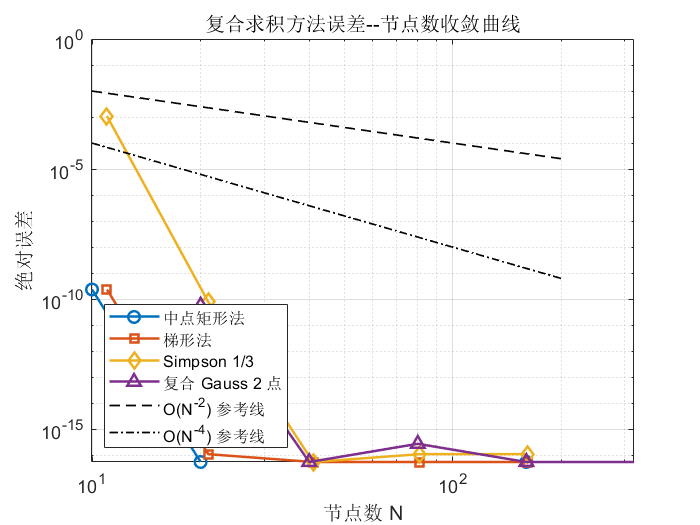
\includegraphics[width=0.9\textwidth]{复合求积方法误差-节点数收敛曲线.png}
    \caption{四种复合求积方法的误差-节点数收敛曲线}
\end{figure}
\subsection{结论}
\begin{table}[H]
    \centering
    \caption{四种复合求积方法的综合比较}
    \label{tab:compare}
    \begin{tabular}{p{2.5cm}p{3.5cm}p{3.5cm}p{3.5cm}}
        \toprule
        维度 & 中矩形 / 梯形法 & Simpson 1/3 & Gauss 2 点 \\
        \midrule
        精度 & $O(h^2)$, 低阶收敛, 需大量节点 & $O(h^4)$, 显著优于低阶方法 & $O(h^4)$, 常数最优, 同节点数下精度最高 \\
        速度 & 均与节点数线性正比；达到相同精度需更多节点, 实际较慢 & 节点数少, 快 & 最快(节点数最少) \\
        实现难度 & 极简, 等距节点 & 简单, 等距节点, 注意奇偶项 & 较复杂, 需非均匀节点与权重(可查表) \\
        信息需求 & 仅需等距节点函数值 & 等距节点函数值 & 必须能在任意给定点计算函数值 \\
    \bottomrule
    \end{tabular}
\end{table}
\appendix
\section{复合求积方法误差--节点数收敛曲线绘图代码}\label{sec:code_convergence_plot}
\begin{lstlisting}
clear; clc; close all;

% 被积函数与高精度参考值
f = @(x) exp(-5*x.^2);
a = 0;  b = 3;
I_exact = integral(f, a, b, 'RelTol',1e-12, 'AbsTol',1e-14);

% 试验的子区间数(逐次加倍)
n_sub = [10, 20, 40, 80, 160];

% 预分配误差数组
err_mid   = zeros(size(n_sub));
err_trap  = zeros(size(n_sub));
err_simp  = zeros(size(n_sub));
err_gauss2 = zeros(size(n_sub));

for i = 1:length(n_sub)
    n = n_sub(i);
    h = (b-a)/n;
    
    % ---- 复合中点矩形法 ----
    x_mid = linspace(a + h/2, b - h/2, n);
    I_mid = h * sum(f(x_mid));
    err_mid(i) = abs(I_mid - I_exact);
    
    % ---- 复合梯形法 ----
    x_trap = linspace(a, b, n+1);
    I_trap = h * ( (f(a)+f(b))/2 + sum(f(x_trap(2:end-1))) );
    err_trap(i) = abs(I_trap - I_exact);
    
    % ---- 复合 Simpson 1/3 法(要求 n 为偶数)----
    if mod(n,2) ~= 0
        n = n+1;
    end
    x_simp = linspace(a, b, n+1);
    fx_simp = f(x_simp);
    I_simp = h/3 * ( fx_simp(1) + fx_simp(end) ...
                     + 4*sum(fx_simp(2:2:end-1)) ...
                     + 2*sum(fx_simp(3:2:end-2)) );
    err_simp(i) = abs(I_simp - I_exact);
    
    % ---- 复合 2 点 Gauss-Legendre 法 ----
    t_g2 = [-1/sqrt(3), 1/sqrt(3)];
    w_g2 = [1, 1];
    x_edges = linspace(a, b, n+1);
    I_gl2 = 0;
    for j = 1:n
        xL = x_edges(j);
        xR = x_edges(j+1);
        mid = (xL + xR)/2;
        half = (xR - xL)/2;
        x_nodes = mid + half * t_g2;
        I_gl2 = I_gl2 + half * sum(w_g2 .* f(x_nodes));
    end
    err_gauss2(i) = abs(I_gl2 - I_exact);
end

% 各方法对应的实际函数求值次数(节点数)
N_mid   = n_sub;
N_trap  = n_sub + 1;
N_simp  = n_sub + 1;
N_gauss = 2 * n_sub;

% 绘制误差-节点数收敛曲线
figure('Color','white');
loglog(N_mid, err_mid, 'o-', 'LineWidth', 1.5, 'MarkerSize', 7);
hold on;
loglog(N_trap, err_trap, 's-', 'LineWidth', 1.5, 'MarkerSize', 7);
loglog(N_simp, err_simp, 'd-', 'LineWidth', 1.5, 'MarkerSize', 7);
loglog(N_gauss, err_gauss2, '^-', 'LineWidth', 1.5, 'MarkerSize', 7);

% 理论收敛阶参考线(斜率 -2 和 -4)
N_ref = [10, 200];
y0_2 = 1e-2 * (N_ref/10).^(-2);
y0_4 = 1e-4 * (N_ref/10).^(-4);
loglog(N_ref, y0_2, 'k--', 'LineWidth', 1);
loglog(N_ref, y0_4, 'k-.', 'LineWidth', 1);

% 图形标注(使用 tex 解释器, 避免 LaTeX 问题)
xlabel('节点数 N', 'FontSize', 12);
ylabel('绝对误差', 'FontSize', 12);
title('复合求积方法误差--节点数收敛曲线', 'FontSize', 14);
legend('中点矩形法', '梯形法', 'Simpson 1/3', '复合 Gauss 2 点', ...
       'O(N^{-2}) 参考线', 'O(N^{-4}) 参考线', ...
       'Location','southwest');
grid on;
set(gca, 'FontSize', 11);
hold off;

% 输出数值
fprintf('节点数序列:\n');
fprintf('中点: %s\n', mat2str(N_mid));
fprintf('梯形: %s\n', mat2str(N_trap));
fprintf('Simpson: %s\n', mat2str(N_simp));
fprintf('Gauss: %s\n', mat2str(N_gauss));
fprintf('\n误差:\n');
disp('中点误差:'); disp(err_mid);
disp('梯形误差:'); disp(err_trap);
disp('Simpson误差:'); disp(err_simp);
disp('Gauss误差:'); disp(err_gauss2);
\end{lstlisting}
\end{document}
